\documentclass{beamer}
\usepackage[utf8]{inputenc}
% make pause work in aligned environment
\makeatletter
\renewrobustcmd{\beamer@@pause}[1][]{%
  \unless\ifmeasuring@%
  \ifblank{#1}%
    {\stepcounter{beamerpauses}}%
    {\setcounter{beamerpauses}{#1}}%
  \onslide<\value{beamerpauses}->\relax%
  \fi%
}
\makeatother

\title{Classificador Ingênuo De Bayes}
\usetheme{Madrid}
\setbeameroption{hide notes}

\begin{document}
\maketitle

\begin{frame}[allowframebreaks]
\frametitle{Overview}
\tableofcontents
\end{frame}

\begin{frame}
\section{Base de Dados}
\frametitle{Base de Dados}
\subsection{Variáveis de Entrada}
\framesubtitle{Variáveis de Entrada}

\begin{columns}
    \begin{column}{0.5\textwidth}
        \begin{itemize}
            \item age
        
            \item job
        
            \item marital
        
            \item education
        
            \item default
        
            \item balance 
        
            \item housing
        
            \item loan
        
     
        \end{itemize}
    \end{column}
    \begin{column}{0.5\textwidth}
        \begin{itemize}
            \item contact
            
            \item day 
        
            \item duration
        
            \item month
        
            \item campaign
            
            \item pdays
        
            \item previous
        
            \item poutcome
        \end{itemize}
    \end{column}
\end{columns}


\end{frame}


\begin{frame}
\frametitle{Base de Dados}
\subsection{Variável de Saída}
\framesubtitle{Variável de Saída}
\begin{itemize}
\item y
\end{itemize}   
\end{frame}

\begin{frame}
\section{Análise Exploratória dos Dados}
\frametitle{Análise Exploratória dos Dados}
\subsection{Descrição Estatística dos Dados}
\framesubtitle{Descrição Estatístisca dos Dados} 
\begin{columns}
\begin{column}{0.5\textwidth}
    \begin{itemize}
        \item count 
        \item unique
        \item top
        \item freq
        \item mean
    \end{itemize}
\end{column}
\begin{column}{0.5\textwidth}
    \begin{itemize}
        \item std
        \item min
        \item 25\%
        \item 50\%
        \item 75\%
        \item max
    \end{itemize}
\end{column}
\end{columns}
\end{frame}
    
\begin{frame}
\frametitle{Análise Exploratória dos Dados}
\subsection{Gráficos}
\framesubtitle{Gráficos}
\begin{columns}
    \begin{column}{0.5\textwidth}
        \begin{figure}[h]
            \caption{Exemplo}
            \centering % para centralizarmos a figura
            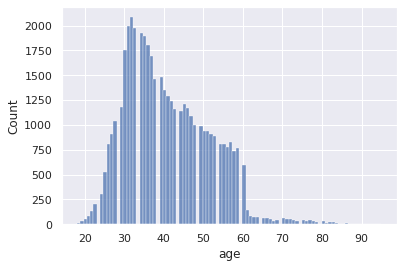
\includegraphics[width=1\textwidth]{IMGS/img1.png}
            \label{figura:distidade}
        \end{figure}
    \end{column}
    \begin{column}{0.5\textwidth}
        \begin{figure}[h]
            \caption{Exemplo2}
            %\centering % para centralizarmos a figura
            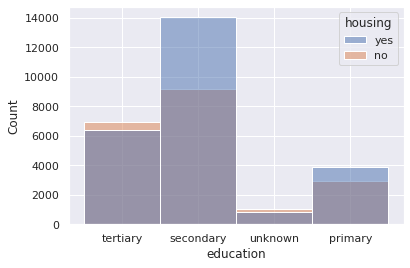
\includegraphics[width=1\textwidth]{IMGS/img2.png}
            \label{figura:fig2}
        \end{figure}
    \end{column}
    \end{columns} 
\end{frame}


\begin{frame}
\frametitle{Análise Exploratória dos Dados}
\framesubtitle{Gráficos}


\begin{columns}
    \begin{column}{0.5\textwidth}
        \begin{figure}[h]
            \caption{Exemplo 3}
            \centering % para centralizarmos a figura
            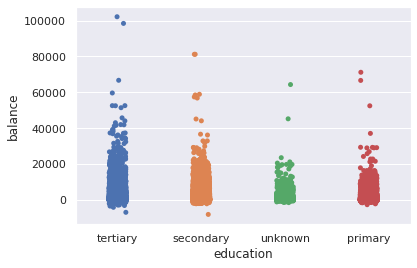
\includegraphics[width=1\textwidth]{IMGS/img3.png}
            \label{figura:distidade}
        \end{figure}
    \end{column}
    \begin{column}{0.5\textwidth}
        \begin{figure}[h]
            \caption{Exemplo 4}
            \centering % para centralizarmos a figura
            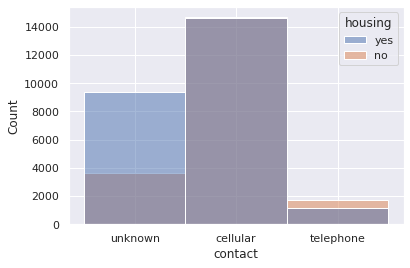
\includegraphics[width=1\textwidth]{IMGS/img4.png}
            \label{figura:fig4}
        \end{figure}
    \end{column}
    \end{columns} 
      
\end{frame}


\begin{frame}
    \frametitle{Análise Exploratória dos Dados}
    \framesubtitle{Gráficos}
    
    
    \begin{columns}
        \begin{column}{0.5\textwidth}
            \begin{figure}[h]
                \caption{Exemplo 5}
                \centering % para centralizarmos a figura
                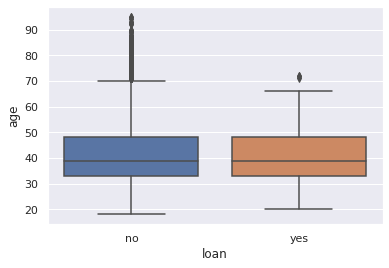
\includegraphics[width=1\textwidth]{IMGS/img5.png}
                \label{figura:distidade}
            \end{figure}
        \end{column}
        \begin{column}{0.5\textwidth}
            \begin{figure}[h]
                \caption{Exemplo 6}
                \centering % para centralizarmos a figura
                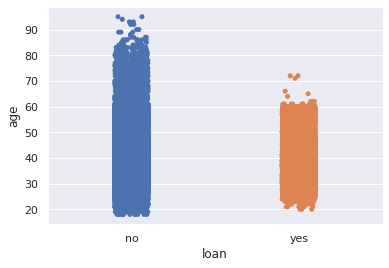
\includegraphics[width=1\textwidth]{IMGS/img6.png}
                \label{figura:fig4}
            \end{figure}
        \end{column}
        \end{columns} 
          
\end{frame}
    
\begin{frame}
    \frametitle{Análise Exploratória dos Dados}
    \framesubtitle{Gráficos}
    
    
    \begin{columns}
        \begin{column}{0.5\textwidth}
            \begin{figure}[h]
                \caption{Exemplo 7}
                \centering % para centralizarmos a figura
                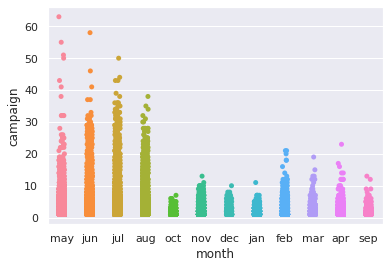
\includegraphics[width=1\textwidth]{IMGS/img7.png}
                \label{figura:distidade}
            \end{figure}
        \end{column}
        \begin{column}{0.5\textwidth}

        \end{column}
        \end{columns} 
          
\end{frame}

\begin{frame}
    \section{Classificador Ingênuo de Bayes}
    \frametitle{Classificador Ingênuo de Bayes}
    \subsection{História}
    \framesubtitle{O que é Naive Bayes}
    
    Baseado no Teorema de Bayes, nome em homenagem ao matemático e pastor presbiteriano inglês Thomas Bayes, que formulou uma função probabilística com o ideal de provar a existência de Deus, é um algoritmo de classificação probabilística muito utilizado para aprendizado de máquina (Machine Learning).
    
\end{frame}

\begin{frame}
\section{Classificador Ingênuo de Bayes}
\frametitle{Classificador Ingênuo de Bayes}
\subsection{Definição Formal do Teorema de Bayes}
\framesubtitle{Definição Formal do Teorema de Bayes}
\begin{equation}
    P(A|B) = \frac{P(B|A)P(A)}{P(B)}
\end{equation}

\begin{itemize}
\item $P(A|B)$ : Probabilidade do evento A ocorrer dado que o evento B ocorreu.
\item $P(B|A)$ : Probabilidade do evento B ocorrer dado que o evento A ocorreu.
\item $P(A)$   : Probabilidade do evento A ocorrer
\item $P(B)$   : Probabilidade do evento B ocorrer. 
\end{itemize}

\end{frame}

\begin{frame}
\frametitle{Classificador Ingênuo de Bayes}
\subsection{Tipos de Classificadores Ingênuo de Bayes}
\framesubtitle{Tipos de Classificadores Ingênuo de Bayes}
\begin{itemize}
\item Bayes Ingênuo Gaussiano
\item Bayes Ingênuo Categórico
\end{itemize}
\end{frame}

\begin{frame}
    \frametitle{Classificador Ingênuo de Bayes}
    \subsection{Vantagens}
    \framesubtitle{Vantagens}
    \begin{itemize}
    \item Rápido
    \item Eficiente
    \item Lida com múltiplos tidos de dados
    \item Ignora características irrelevantes
    
    \end{itemize}
    \end{frame}
    \begin{frame}
    \frametitle{Classificador Ingênuo de Bayes}
    \subsection{Desvantagens}
    \framesubtitle{Desvantagens}
    \begin{itemize}
    \item Previsão falha em frequência zero
    \item Ignorar a correlação entre as variáveis
    \end{itemize}
    \end{frame}

\begin{frame}
\frametitle{Classificador Ingênuo de Bayes}
\subsection{Sobre o Projeto}
\framesubtitle{Sobre o Projeto}
\begin{figure}[H]
    \centerline{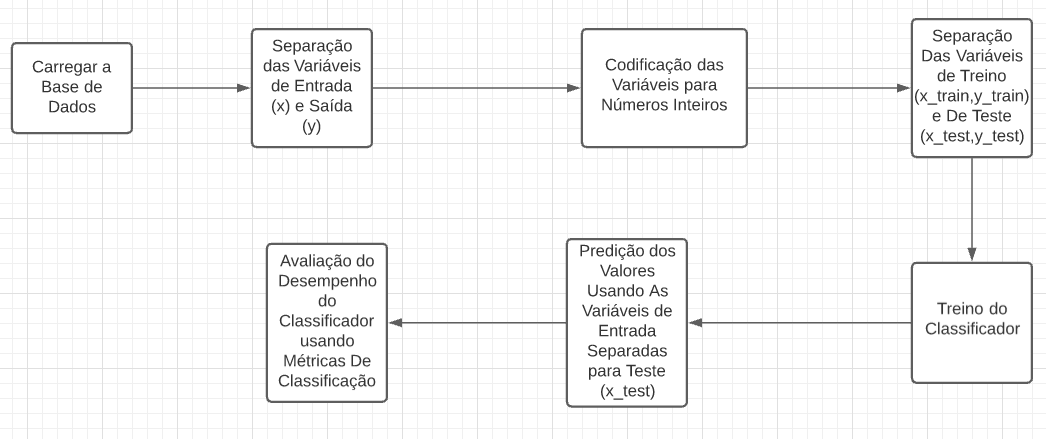
\includegraphics[width=1.0\textwidth]{IMGS/block1.png}}
\end{figure}    
\end{frame}


\begin{frame}
\section{Experimentos} 
\frametitle{Experimentos}
\subsection{Experimentos Iniciais}
\framesubtitle{Experimentos Iniciais}
\begin{itemize}
\item Precision:
\begin{equation}
    \frac{t_p}{t_p + f_p}
\end{equation}
\item Accuracy
\begin{equation}
    \frac{t_p + t_n}{t_p + t_n + f_p + f_n}
\end{equation}
\item Recall Score
\begin{equation}
    \frac{t_p}{t_p + f_n}
\end{equation}
\item F1 Score
\begin{equation}
    \frac{2\cdot(precision\cdot recall)}{precision +  recall}
\end{equation}
\end{itemize}
\end{frame}





\begin{frame}
\frametitle{Experimentos}
\framesubtitle{Experimentos Iniciais}
\begin{table}[H]
    \centering
    \begin{small}
        \begin{tabular}{ccc}
            \\
            %\multicolumn{2}{c}{{\fontsize{13}{\baselineskip} \selectfont C}{\fontsize{11}{\baselineskip}\selectfont RONOGRAMA DE}{\fontsize{13}{\baselineskip} \selectfont A}{\fontsize{11}{\baselineskip}\selectfont TIVIDADES }}\\ 
            \\
            \hline
                                    & Categórico       & Gaussiano\\
            \hline
            Precision               & 0.89             & 0.84\\
            Accuracy                & 0.89             & 0.84\\
            Recall Score            & 0.89             & 0.84\\
            F1-Score                & 0.89             & 0.84\\
            
            \hline
        \end{tabular}
    \end{small}
\end{table}
    \begin{columns}
        \begin{column}{0.5\textwidth}
            \begin{table}[H]

                \centering
                \caption{\label{tab:cr1-cnb} Relatório de Classificação por Label do Classificador Categórico.}
                \begin{small}
                    \begin{tabular}{ccc}
                    
                        \hline
                                                & 0                & 1\\
                        \hline
                        Precision               & 0.93             & 0.53\\
                        Recall Score            & 0.95             & 0.43\\
                        F1-Score                & 0.94             & 0.47\\
                        
                        \hline
                    \end{tabular}
                \end{small}
            
            \end{table}
        \end{column}
        \begin{column}{0.5\textwidth}
            \begin{table}[H]

                \centering
                \caption{\label{tab:cr1-gnb} Relatório de Classificação por Label do Classificador Gaussiano}
                \begin{small}
                    \begin{tabular}{ccc}
                    
                        \hline
                                                & 0                & 1\\
                        \hline
                        Precision                & 0.89             & 0.49\\
                        Recall Score            & 1.00             & 0.03\\
                        F1-Score                & 0.94             & 0.06\\
                        
                        \hline
                    \end{tabular}
                \end{small}
            
            \end{table}
        \end{column}
        \end{columns}    
\end{frame}

\begin{frame}
    \frametitle{Experimentos}
    \framesubtitle{Experimentos Iniciais}
    \begin{columns}
        \begin{column}{0.5\textwidth}
            \begin{figure}[H]
                \centerline{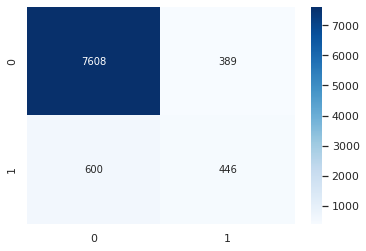
\includegraphics[width=1.0\textwidth]{IMGS/cm-categorico.png}}
                
                \caption{\label{fig:cm1-cnb}Confusion Matrix do Classificador Categórico}
                \end{figure}
        \end{column}
        \begin{column}{0.5\textwidth}
            \begin{figure}[H]
                \centerline{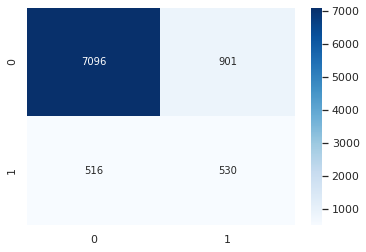
\includegraphics[width=1.0\textwidth]{IMGS/cm-gaussiano.png}}
                \label{cm1-gnb}
                \caption{\label{fig:cm1-gnb}Confusion Matrix do Classificador Gaussiano}
                \end{figure}
        \end{column}
        \end{columns}    
\end{frame}







\begin{frame}
    \frametitle{Experimentos}
    \subsection{Usando Apenas a Variável Age para Treino}
    \framesubtitle{Usando Apenas a Variável Age para Treino}
    \begin{table}[H]
        \centering
        \begin{small}
            \begin{tabular}{ccc}
                \\
                %\multicolumn{2}{c}{{\fontsize{13}{\baselineskip} \selectfont C}{\fontsize{11}{\baselineskip}\selectfont RONOGRAMA DE}{\fontsize{13}{\baselineskip} \selectfont A}{\fontsize{11}{\baselineskip}\selectfont TIVIDADES }}\\ 
                \\
                \hline
                                        & Categórico       & Gaussiano\\
                \hline
                Precision               & 0.88             & 0.88\\
                Accuracy                & 0.88             & 0.88\\
                Recall Score            & 0.88             & 0.88\\
                F1-Score                & 0.88             & 0.88\\
                
                \hline
            \end{tabular}
        \end{small}
    \end{table}
        \begin{columns}
            \begin{column}{0.5\textwidth}
                \begin{table}[H]

                    \centering
                    \caption{\label{tab:cr2-cnb} Relatório de Classificação por Label do Classificador Categórico.}
                    \begin{small}
                        \begin{tabular}{ccc}
                        
                            \hline
                                                    & 0                & 1\\
                            \hline
                            Precision               & 0.88             & 0.50\\
                            Recall Score            & 1.00             & 0.02\\
                            F1-Score                & 0.94             & 0.04\\
                            
                            \hline
                        \end{tabular}
                    \end{small}
                \end{table}
            \end{column}
            \begin{column}{0.5\textwidth}
                \begin{table}[H]

                    \centering
                    \caption{\label{tab:cr2-gnb} Relatório de Classificação por Label do Classificador Gaussiano}
                    \begin{small}
                        \begin{tabular}{ccc}
                        
                            \hline
                                                    & 0                & 1\\
                            \hline
                            Precision               & 0.88             & 0.48\\
                            Recall Score            & 1.00             & 0.03\\
                            F1-Score                & 0.94             & 0.05\\
                            
                            \hline
                        \end{tabular}
                    \end{small}
                
                \end{table}
            \end{column}
            \end{columns}    
    \end{frame}
    
\begin{frame}
    \frametitle{Experimentos}
    \framesubtitle{Usando Apenas a Variável Age para Treino}
    \begin{columns}
        \begin{column}{0.5\textwidth}
            \begin{figure}[H]
                \centerline{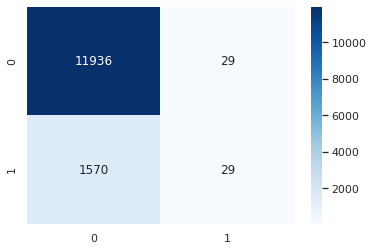
\includegraphics[width=1.0\textwidth]{IMGS/cm-cnb-age-only.png}}
                
                \caption{\label{fig:cm2-cnb}Confusion Matrix do Classificador Categórico}
            \end{figure}
        \end{column}
        \begin{column}{0.5\textwidth}
            \begin{figure}[H]
                \centerline{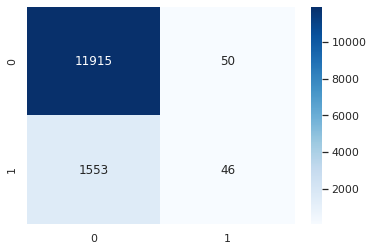
\includegraphics[width=1.0\textwidth]{IMGS/cm-gnb-age-only.png}}
                \caption{\label{fig:cm2-gnb}Confusion Matrix do Classificador Gaussiano}
            \end{figure}
        \end{column}
        \end{columns}    
\end{frame}





\begin{frame}
    \frametitle{Experimentos}
    \subsection{Usando Apenas Variáveis Numéricas Para Treino}
    \framesubtitle{Usando Apenas Variáveis Numéricas Para Treino}
    \begin{table}[H]
        \centering
        \caption{\label{tab:cr3-gt} Comparação entre o Classificador Categórico e o Gaussiano}
        \begin{small}
            \begin{tabular}{ccc}
                \\
                %\multicolumn{2}{c}{{\fontsize{13}{\baselineskip} \selectfont C}{\fontsize{11}{\baselineskip}\selectfont RONOGRAMA DE}{\fontsize{13}{\baselineskip} \selectfont A}{\fontsize{11}{\baselineskip}\selectfont TIVIDADES }}\\ 
                \\
                \hline
                                        & Categórico       & Gaussiano\\
                \hline
                Precision               & 0.89             & 0.89\\
                Accuracy                & 0.89             & 0.89\\
                Recall Score            & 0.89             & 0.89\\
                F1-Score                & 0.89             & 0.89\\
                
                \hline
            \end{tabular}
        \end{small}
    \end{table}


        \begin{columns}
            \begin{column}{0.5\textwidth}
                \begin{table}[H]
                    \caption{\label{tab:cr3-cnb} Relatório de Classificação por Label do Classificador Categórico.}
                    \centering
                    \begin{small}
                        \begin{tabular}{ccc}
                        
                            \hline
                                                    & 0                & 1\\
                            \hline
                            Precision               & 0.89             & 0.63\\
                            Recall Score            & 0.99             & 0.11\\
                            F1-Score                & 0.94             & 0.18\\
                            
                            \hline
                        \end{tabular}
                    \end{small}
                \end{table}
            \end{column}
            \begin{column}{0.5\textwidth}
                \begin{table}[H]

                    \centering
                    \caption{\label{tab:cr3-gnb} Relatório de Classificação por Label do Classificador Gaussiano}
                    \begin{small}
                        \begin{tabular}{ccc}
                        
                            \hline
                                                    & 0                & 1\\
                            \hline
                            Precision               & 0.91             & 0.53\\
                            Recall Score            & 0.96             & 0.32\\
                            F1-Score                & 0.94             & 0.40\\
                            
                            \hline
                        \end{tabular}
                    \end{small}
                
                \end{table}
            \end{column}
            \end{columns}    
    \end{frame}
    
\begin{frame}
    \frametitle{Experimentos}
    \framesubtitle{Usando Apenas Variáveis Numéricas Para Treino}
    \begin{columns}
        \begin{column}{0.5\textwidth}
            \begin{figure}[H]
                \centerline{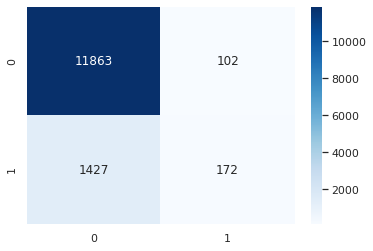
\includegraphics[width=1.0\textwidth]{IMGS/cm-cnb-numeric.png}}
                
                \caption{\label{fig:cm3-cnb}Confusion Matrix do Classificador Categórico}
            \end{figure}
            
        \end{column}
        \begin{column}{0.5\textwidth}
            \begin{figure}[H]
                \centerline{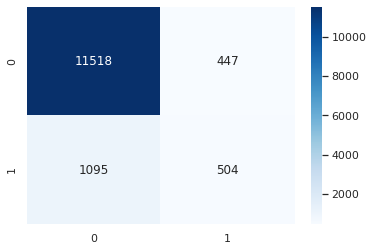
\includegraphics[width=1.0\textwidth]{IMGS/cm-gnb-numeric.png}}
                \caption{\label{fig:cm3-gnb}Confusion Matrix do Classificador Gaussiano}
            \end{figure}
        \end{column}
        \end{columns}    
\end{frame}

\begin{frame}
\section{Análise dos Resultados}
\subsection{Resultados Iníciais}
\frametitle{Análise dos Resultados}
\framesubtitle{Resultados Iniciais}  
\begin{itemize}
\item Classificador Gaussiano vs Classificador Categórico
\item Número de Features
\item Falsos positivos vs Falsos Negativos
\end{itemize}
\end{frame}

\begin{frame}
    \frametitle{Análise dos Resultados}  
    \subsection{Perfil Mais Receptivo}
    \framesubtitle{Perfil Mais Receptivo}
    \begin{itemize}
    \item Profissão: estudante
    \item Estado Civil: divorciado
    \item Credito Pessoal: possui
    \item Credito de Habitação: não possui
    \item Tipo de Contato: celular
    \item Educação: ensino médio
    \item Mês da Campanha: setembro
    \end{itemize}
\end{frame}

\begin{frame}
    \frametitle{Análise dos Resultados}  
    \subsection{Perfil Menos Receptivo}
    \framesubtitle{Perfil Menos Receptivo}
    \begin{itemize}
    \item Profissão: operario
    \item Estado Civil: casado
    \item Credito Pessoal: não possui
    \item Credito de Habitação: possui
    \item Tipo de Contato: unknown
    \item Educação: ensino fundamental
    \item Mês da Campanha: maio
    \end{itemize}
\end{frame}


\begin{frame}
	\frametitle{Análise dos Resultados}
    \subsection{Categorias exóticas}
	\framesubtitle{Categorias exóticas}
	\begin{columns}
		\begin{column}{1\textwidth}
			\begin{figure}[H]
				\centerline{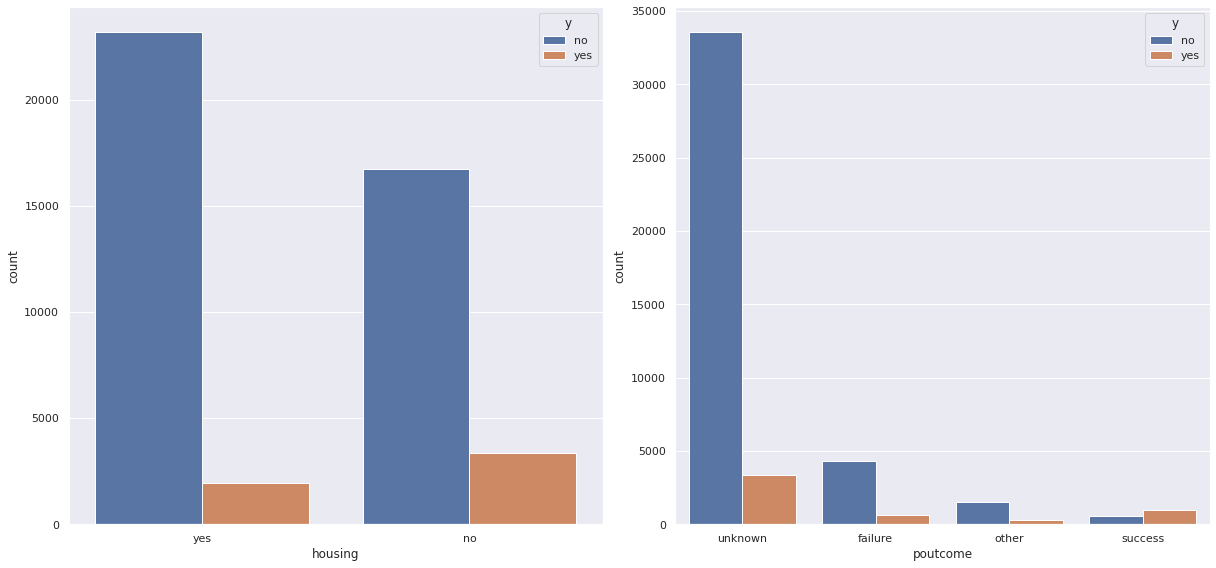
\includegraphics[width=1.0\textwidth]{IMGS/analise1.png}}
				
				\caption{\label{fig:analise1}Categorias mais exóticas}
			\end{figure}
		\end{column}
	\end{columns}    
\end{frame}
\end{document}
